\documentclass{beamer}
\mode<presentation>
\usepackage{amsmath,amssymb,mathtools}
\usepackage{textcomp}
\usepackage{gensymb}
\usepackage{adjustbox}
\usepackage{subcaption}
\usepackage{enumitem}
\usepackage{multicol}
\usepackage{listings}
\usepackage{url}
\usepackage{graphicx} % <-- needed for images
\def\UrlBreaks{\do\/\do-}

\usetheme{Boadilla}
\usecolortheme{lily}
\setbeamertemplate{footline}{
  \leavevmode%
  \hbox{%
  \begin{beamercolorbox}[wd=\paperwidth,ht=2ex,dp=1ex,right]{author in head/foot}%
    \insertframenumber{} / \inserttotalframenumber\hspace*{2ex}
  \end{beamercolorbox}}%
  \vskip0pt%
}
\setbeamertemplate{navigation symbols}{}

\lstset{
  frame=single,
  breaklines=true,
  columns=fullflexible,
  basicstyle=\ttfamily\tiny   % tiny font so code fits
}

\numberwithin{equation}{section}

% ---- your macros ----
\providecommand{\nCr}[2]{\,^{#1}C_{#2}}
\providecommand{\nPr}[2]{\,^{#1}P_{#2}}
\providecommand{\mbf}{\mathbf}
\providecommand{\pr}[1]{\ensuremath{\Pr\left(#1\right)}}
\providecommand{\qfunc}[1]{\ensuremath{Q\left(#1\right)}}
\providecommand{\sbrak}[1]{\ensuremath{{}\left[#1\right]}}
\providecommand{\lsbrak}[1]{\ensuremath{{}\left[#1\right.}}
\providecommand{\rsbrak}[1]{\ensuremath{\left.#1\right]}}
\providecommand{\brak}[1]{\ensuremath{\left(#1\right)}}
\providecommand{\lbrak}[1]{\ensuremath{\left(#1\right.}}
\providecommand{\rbrak}[1]{\ensuremath{\left.#1\right)}}
\providecommand{\cbrak}[1]{\ensuremath{\left\{#1\right\}}}
\providecommand{\lcbrak}[1]{\ensuremath{\left\{#1\right.}}
\providecommand{\rcbrak}[1]{\ensuremath{\left.#1\right\}}}
\theoremstyle{remark}
\newtheorem{rem}{Remark}
\newcommand{\sgn}{\mathop{\mathrm{sgn}}}
\providecommand{\abs}[1]{\left\vert#1\right\vert}
\providecommand{\res}[1]{\Res\displaylimits_{#1}}
\providecommand{\norm}[1]{\lVert#1\rVert}
\providecommand{\mtx}[1]{\mathbf{#1}}
\providecommand{\mean}[1]{E\left[ #1 \right]}
\providecommand{\fourier}{\overset{\mathcal{F}}{ \rightleftharpoons}}
\providecommand{\system}{\overset{\mathcal{H}}{ \longleftrightarrow}}
\providecommand{\dec}[2]{\ensuremath{\overset{#1}{\underset{#2}{\gtrless}}}}
\newcommand{\myvec}[1]{\ensuremath{\begin{pmatrix}#1\end{pmatrix}}}
\newcommand{\mydet}[1]{\ensuremath{\begin{vmatrix}#1\end{vmatrix}}}

\newenvironment{amatrix}[1]{%
  \left(\begin{array}{@{}*{#1}{c}|*{#1}{c}@{}}
}{%
  \end{array}\right)
}

\newcommand{\myaugvec}[2]{\ensuremath{\begin{amatrix}{#1}#2\end{amatrix}}}
\let\vec\mathbf
% ---------------------

\title{Matgeo Presentation - Problem 10.6.11}
\author{ee25btech11056 - Suraj.N}

\begin{document}

\begin{frame}
  \titlepage
\end{frame}

\begin{frame}{Problem Statement}

Draw a circle of radius $4\,$cm. Draw two tangents to the circle inclined at an angle of $60^\circ$ to each other.

\end{frame}

\begin{frame}{Data}

\begin{table}[h!]
  \centering
  \begin{tabular}{|c|c|}
\hline
\textbf{Name} & \textbf{Value} \\ \hline
$\vec{A}$ & $\myvec{2 & 1 \\0 & 3}$ \\ \hline
\end{tabular}

  \caption*{Table : Circle}
  \label{10.6.11}
\end{table}

\end{frame}

\begin{frame}{Solution}

The parameters of the circle with center $\vec{0}$ are :

\begin{align}
  \vec{V} &= \vec{I} & \vec{u} &= \vec{0} & f &= -16
\end{align}

Let the point from which tangent is being drawn be $\vec{p}$ .\\

Let the point of contact be $\vec{q}$ and 

\begin{align}
\vec{q}^\top\vec{q} = 16 
\end{align}

From the condition of tangency we get 

\begin{align}
  \vec{q}^\top(\vec{q}-\vec{p}) &= 0\\
  \vec{p}^\top\vec{q} &= \vec{q}^\top\vec{q}\\
  \vec{p}^\top\vec{q} &= 16 \label{eq:pq} 
\end{align}

If the angle between the tangents is 60{\degree} then the angle betweent the normals at the points of contact is 120{\degree}.\\


\end{frame}

\begin{frame}{Solution}


Therefore,

\begin{align}
  \cos(\tfrac{120\degree}{2}) &= \frac{\vec{p}^\top\vec{q}}{\norm{\vec{p}}\norm{\vec{q}}}\\
  \norm{\vec{p}} &= 8\\
  \vec{p}^\top\vec{p} - 64 &= 0
\end{align}

Therefore the locus of point $\vec{p}$ is a circle with center $\vec{0}$ and radius 8 cm.\\

Consider point $\vec{P} = \myvec{8\\0}$ (lies on the locus) from which tangents are drawn.\\

Let the tangent equation passing through $\vec{P}$ be 

\begin{align}
  \vec{x} &= \vec{P} + k\vec{m}
\end{align}

\end{frame}

\begin{frame}{Solution}

Finding the point of contact :

\begin{align}
  g(\vec{x}) = \vec{x}^\top\vec{x} - 16 \label{eq:circle}\\
  (\vec{P}+k\vec{m})^\top(\vec{P}+k\vec{m}) - 16 = 0\\
  k^2\vec{m}^\top\vec{m} + 2k\vec{P}^\top\vec{m} + \vec{P}^\top\vec{P} - 16 = 0\\
  k^2\vec{m}^\top\vec{m} + 2k\vec{P}^\top\vec{m} + g(\vec{P}) = 0\\
\end{align}
As the tangent intersects the conic at only one point(the point of contact),the discriminant for the quadratic in k is equal to 0
\begin{align}
    g(\vec{P}) = 48\\
  \vec{m}^\top\myvec{-16 & 0\\0 & 48}\vec{m} = 0 \label{eq:mqm} \\
  \vec{Q} = \myvec{-16 & 0\\0 & 48}\\ 
\end{align}

\end{frame}

\begin{frame}{Solution}

As $\vec{Q}$ is an upper triangular matrix , the eigen values are the diagonal entries :

\begin{align}
  \lambda_1 &= -16 & \lambda_2 &= 48
\end{align}

Applying eigen value decomposition for $\vec{Q}$ 

\begin{align}
  \vec{Q} = \vec{X}\vec{D}\vec{X}^\top\\
  \vec{D} = \myvec{-16 & 0\\0 & 48}
\end{align}

$\vec{X}$ is an orthogonal matrix whose columns are the corresponding normalized eigenvectors of $\vec{Q}$\\
As $\vec{Q}$ is a diagonal matrix , 

\begin{align}
  \vec{X} = \vec{I}
\end{align}

\end{frame}

\begin{frame}{Solution}

From \eqref{eq:mqm} ,

\begin{align}
  \vec{m}^\top\vec{X}\vec{D}\vec{X}^\top\vec{m} = 0\\
  \vec{z} = \vec{X}^\top\vec{m}\\
  \vec{z}^\top\vec{D}\vec{z} = 0\\
  \myvec{z_1 & z_2}\myvec{-16 & 0\\0 & 48}\myvec{z_1\\z_2} = 0\\
  \frac{z_1}{z_2} = \pm \sqrt{3} \label{eq:z} 
\end{align}

Solving for $\vec{m}$ ,
\begin{align}
  \vec{I}\vec{m} = \vec{z}\\
  \vec{m} = \myvec{z_1\\z_2}\\
  \vec{m} = \myvec{1\\\tfrac{z_2}{z_1}}
\end{align}

\end{frame}

\begin{frame}{Solution}

From \eqref{eq:z} , the direction vectors for the tangents are given as :

\begin{align}
  \vec{m_1} &= \myvec{1\\\tfrac{1}{\sqrt{3}}} & \vec{m_2} &= \myvec{1\\-\tfrac{1}{\sqrt{3}}}
\end{align}

The normal vectors for the tangents are given as :

\begin{align}
  \vec{n_1} &= \myvec{-\tfrac{1}{\sqrt{3}}\\1} & \vec{n_2} &= \myvec{\tfrac{1}{\sqrt{3}}\\1} 
\end{align}

The points of contacts are given as :

\begin{align}
  \vec{q_i} &= \pm r \frac{\vec{n_i}}{\norm{\vec{n_i}}}
\end{align}

From \eqref{eq:pq} , $\vec{P}^\top\vec{q}=16$ , so the points of contact are :
\begin{align}
  \vec{q_1} &= \myvec{2\\2\sqrt{3}} & \vec{q_2} &= \myvec{2\\-2\sqrt{3}}
\end{align}

\end{frame}

\begin{frame}{Plot}

\begin{figure}[h!]
  \centering
  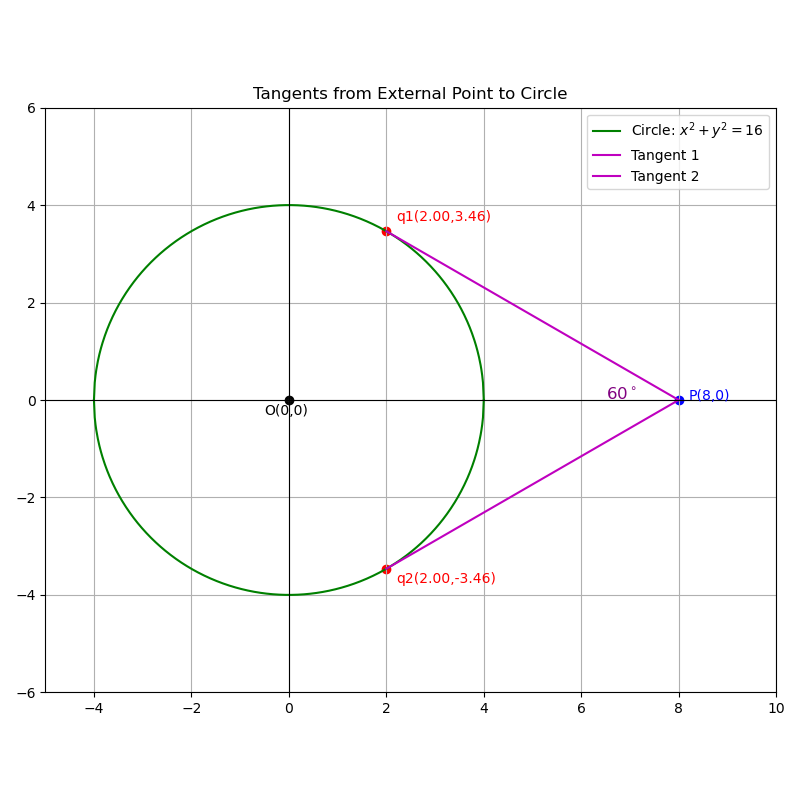
\includegraphics[width=0.6\columnwidth]{figs/circle_tangents.png} 
   \caption*{Fig : Circle and Tangents}
  \label{Fig1}
\end{figure}

\end{frame}

\end{document}


